\chapter{Nmpc-codegen}
This chapter describes the software library that was written with this thesis. First an overview of the workflow and the functionality of the library is given. Followed by a more in-depth description of the implementation.
\section{Overview library}
The nmpc-codegen library contains a framework to construct a Python or Matlab script that generates a MPC controller. This controller uses the PANOC algorithm to solve its NLP problem.

Figure~\eqref{fig:nmpc-codegen scheme} illustrates the different parts of a typical script . On the left side is the Python or Matlab script that the user will construct. It contains the mathematical model and the control parameters of the process that needs to be controlled.The output of the Python/Matlab script is displayed on the right side in figure~\ref{fig:nmpc-codegen scheme}. The output contains some static code, which is mostly associated with the PANOC algorithm. And some dynamic code which is generated in Python or Matlab which will differ depending on the problem. Sometimes the output will also contain simulation tools. These simulation tools exsist of a Python, Matlab interface and a build system to compile itself. It allows the user to simulate the controller from within Python or Matlab.
	\begin{figure}[H]
		\centering
		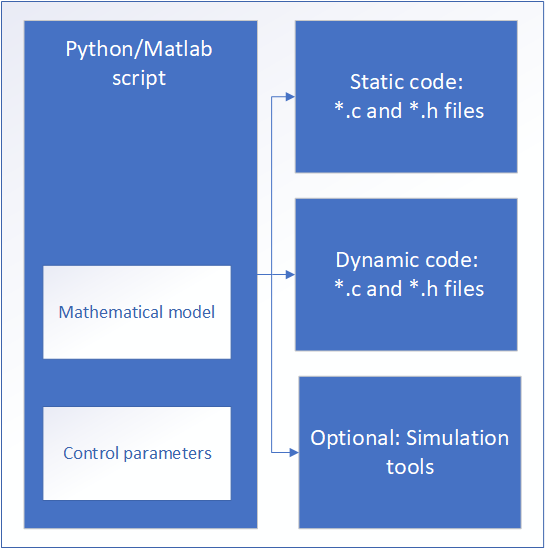
\includegraphics[width=0.5\textwidth]{nmpc_codegen_scheme}
		\caption{Nmpc-codegen scheme}
		\label{fig:nmpc-codegen scheme}
	\end{figure}

\section{Casadi}
The PANOC algorithm is a derivative driven algorithm, this means that the gradient of the cost function must be available to the algorithm. This gradient is generated using backward automatic differentiation.

\subsection{Algorithmic differentiation (AD)}
There exists a number of ways to determine the derivative of a function. The most obvious way is using symbolic differentiation. This method has been used over more than 200 years to calculate the gradient by hand. But in order to use symbolic differentiation, the algorithm needs one mathematical defined function. Which might be hard to realize in practice.

Another way of calculating derivatives, is through numerical differentiation also known as the method of finite differences. Although this method is very simple to implement, the accuracy is not always sufficient. And the method is rather slow if there are lots of partial derivatives.

A second alternative way to symbolic differentiation is through automatic differentiation. This method has two variants forward automatic differentiation and backward automatic differentiation.

The entire function must be expressed in elementary operations in order to use automatic differentiation. This is something computers are naturally good at. \eqref{eq:example used with automatic differentiation} Illustrates a simple example of such function. Two intermediate valuables are used to express the elementary operations.
\begin{equation}
	\begin{aligned}
		& y = a \cdot b + cos(b) \\
		& x_1 = a \cdot b \\
		& x_2 = cos(b) \\
		& y = x_1 + x_2		
	\end{aligned}
	\label{eq:example used with automatic differentiation}
\end{equation}
Forward automatic differentiation gets its name from the fact that the chain rule is applied from input to output. It derives going from the lowest variables to the highest viable, as illustrated by \eqref{eq:math definition forward automatic differentiation}. \eqref{eq:example forward automatic differentiation} Contains a worked out example of this algorithm. The first line of \eqref{eq:example forward automatic differentiation} contains the theoretical answer. The  following two lines contain the derivatives of the two intermediate variables towards the b variable. Finally the two separate derivatives are summed up to obtain the complete derivative towards b.

When using forward automatic differentiation, each element of the gradient has its own intermediate derivatives that need to be calculated. This is where the idea for backward automatic differentiation came from. As it generates the derivative towards all inputs variables in one big sweep. Although it's more expensive to calculate one single derivative of the gradient, it is cheaper to calculate the entire gradient.

\begin{equation}
	\frac{dx_i}{db} = \frac{dx_i}{dx_j}\frac{dx_j}{dx_k}\frac{dx_k}{db}
	\label{eq:math definition forward automatic differentiation}
\end{equation}

\begin{equation}
	\begin{aligned}
		& \frac{\partial y}{\partial b} = a - sin(b) \\
		& \frac{\partial x_1}{\partial b} = a  \\
		& \frac{\partial x_2}{\partial b} = -sin(b) \\
		& \frac{\partial y}{\partial b} = \frac{\partial x_1}{\partial b} + \frac{\partial x_2}{\partial b}	 = a - sin(b)
	\end{aligned}
	\label{eq:example forward automatic differentiation}
\end{equation}

Backward automatic differentiation as described in\cite{Dhiel} is the opposite of forward automatic differentiation, as it works down from the output towards the input. As illustrated by \eqref{eq:math definition backward automatic differentation}. An example is worked out in \eqref{eq:example backward automatic differentiation}. Even if there are hundreds of intermediate variables it only requires only one sweep to find all the components of the gradient. This is the main reason why packages like Casadi use backward automatic differentiation, instead of forward automatic differentiation.

\begin{equation}
	\frac{\partial x_i}{\partial b} = \frac{\partial x_i}{\partial x_k}\frac{\partial x_k}{\partial x_j}\frac{\partial x_j}{\partial b}
	\label{eq:math definition backward automatic differentation}
\end{equation}

\begin{equation}
\begin{aligned}
& \bar{x_1} = \bar{x_3} \frac{\partial x_3}{\partial x_1} = 1 \cdot 1 \\
& \bar{x_2} = \bar{x_3} \frac{\partial x_3}{\partial x_2} = 1 \cdot 1 \\
& \frac{\partial y}{\partial b} = \bar{x_1} \frac{\partial x_1}{\partial b} + \bar{x_2} \frac{\partial x_2}{\partial b} = a - sin(b)\\
& \frac{\partial y}{\partial a} = \bar{x_1} \frac{\partial x_1}{\partial a} = b
\end{aligned}
\label{eq:example backward automatic differentiation}
\end{equation}

The same example can be calculated with Casadi as demonstrated in listing~\ref{lst:casadi demo backward automatic differentiation} with output in table~\ref{tbl:output casadi demo backward automatic differentiation}. The intermediate variables are @1,@2 and @3. output[0][0] is the function value and input[1][0] and input[1][1] is the gradient. 

\begin{lstlisting}[caption={Casadi code example automatic backward differentiation},label={lst:casadi demo backward automatic differentiation}]
a = cd.SX.sym('a',(1,1))
b = cd.SX.sym('b',(1,1))
y = a*b + cd.cos(b)
f = cd.Function('f',[a,b],[y,cd.gradient(y,cd.vertcat(a,b))])
print(f)
\end{lstlisting}


\begin{table}
	\begin{center}
		\begin{tabular}{ |l|  }
			\hline
			Output Casadi code listing~\ref{lst:casadi demo backward automatic differentiation} \\
			\hline
			Number of inputs: 2 \\
			Input 0 ("i0"): 1-by-1 (dense) \\
			Input 1 ("i1"): 1-by-1 (dense) \\
			Number of outputs: 2 \\
			Output 0 ("o0"): 1-by-1 (dense) \\
			Output 1 ("o1"): 2-by-1 (dense) \\
			@0 = input[0][0]; \\
			@1 = input[1][0]; \\
			@2 = (@0*@1); \\
			@3 = cos(@1); \\
			@2 = (@2+@3); \\
			output[0][0] = @2; \\
			output[1][0] = @1; \\
			@1 = sin(@1); \\
			@0 = (@0-@1); \\
			output[1][1] = @0; \\
			\hline   
		\end{tabular}
		\caption{output casadi demo backward automatic differentiation}
		\label{tbl:output casadi demo backward automatic differentiation}
	\end{center}
\end{table}


\section{Nmpc-codegen implementation}
Nmpc-codegen is constructed out of a high-level language such as Python or Matlab that generates header files and source files. In order to test the controller, the high-level language can call the build system (Cmake/make) to compile the generate code. And then simulate the controller to see the response.

\subsection{Python and Matlab}
Figure~\ref{fig:nmpc_codegen_packages} illustrates the architecture of the nmpc-codegen library. There are five sub packages: tools, models, example models, controller and Cfunctions.  The two classes in the sub package models, represent the mathematical model of the system. The user must construct an object of one of these classes, that contains the function equation of the system.

The Cfunctions sub package contains proximal functions that represent constraints on the inputs. The user manual contains a table of all available constraints to the user. The tools sub package contains two classes. The bootstrapper that can generate the static code, and the simulator that allows the user to call the generated C code from Python or Matlab.

The controller sub package contains the Nmpc\_PANOC class, an object of this class represents the actual controller. In order to construct an object of the Nmpc\_PANOC class the user must provide: a model object, a proximal function object and one or two stage costs object.

Finally the user can also add obstacles or constraints, these can be added as soft constraints onto the cost function. The obstacles/constraints can be found in the sub package obstacles/constraints from the sub package controller. The final chapter discusses an alternative way to add constraints using a Lagrangian.
	\begin{figure}[H]
		\centering
		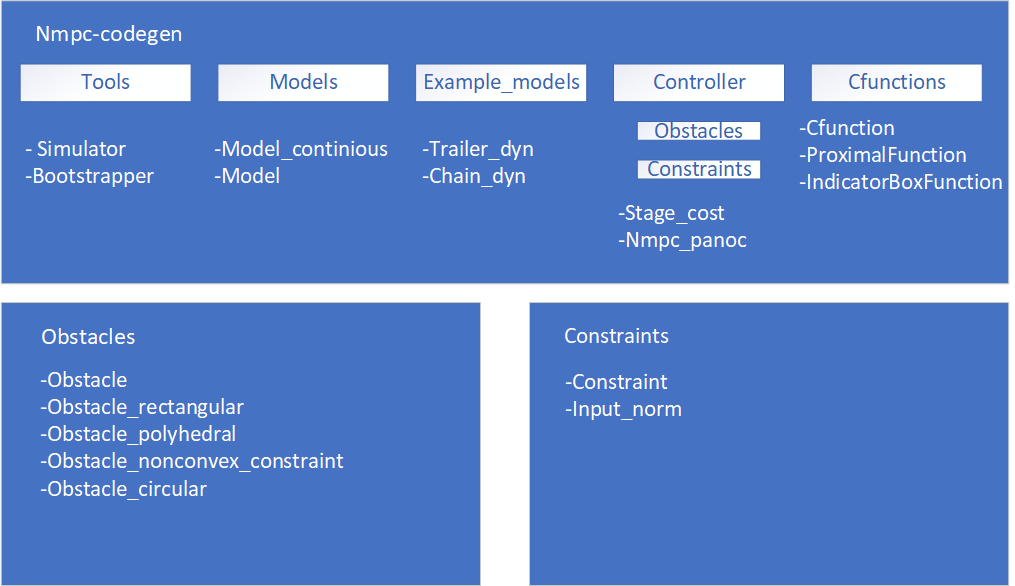
\includegraphics[width=1\textwidth]{nmpc_codegen_packages}
		\caption{Software architecture Python/Matlab}
		\label{fig:nmpc_codegen_packages}
	\end{figure}

\subsection{C}
The C code is written in a layered architecture, the lowest layer contains the buffer, the cost function and the lipschitz estimator. The second layer contains the proximal gradient algorithm and the L-BFGS algorithm. The highest layer contains the PANOC algorithm as illustrated in figure~\ref{fig:visio software arch}.

The NMPC entity initializes the cost function with the current state of each iteration, and calls PANOC repeatably till convergence. The end-user does not need to know how PANOC or any of the underlying layers work. The NMPC entity takes care of everything, the user will simply call NMPC with the current state, a reference state, a reference input and an output array to place the optimal inputs in.

	\begin{figure}[H]
		\centering
		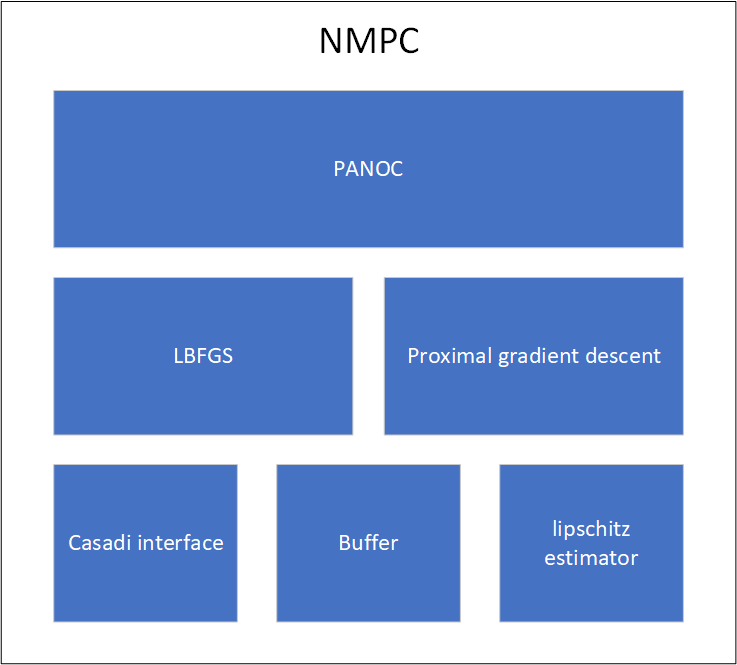
\includegraphics[width=0.5\textwidth]{visio_software_arch}
		\caption{Software architecture C code}
		\label{fig:visio software arch}
	\end{figure}

\subsection{Build system}
The build system to compile the Python/Matlab interface is compatible with Windows, Linux and Mac X os. Cmake is able to generate build systems for all three opening systems, and was the obvious choice as it is used by many other open-source projects. The structure of the build system is illustrated in figure~\ref{fig:build system}. Python or Matlab first calls Cmake to generate the Make files. After the Make files are generated the Python or Matlab code calls the makefile to compile the controller code into a shared library.
\begin{figure}[H]
	\centering
	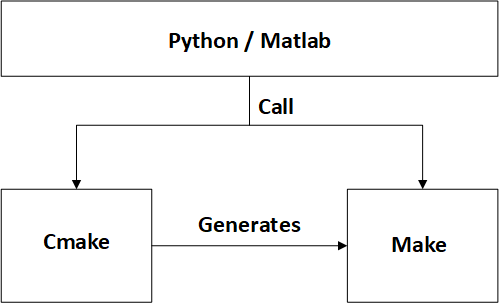
\includegraphics[width=0.5\textwidth]{build_system}
	\caption{Build system}
	\label{fig:build system}
\end{figure}
After the dynamic library is compiled, the Python code must call the functions inside the dynamic library. This is accomplished using the Ctypes library, which allows Python scripts to directly call C functions from a dynamic library with the right properties.

Matlab can also call directly into a dynamic library, this is accomplished through the callib function in Matlab. So the same compiled shared library can be used for either Matlab or Python.

\subsection{How to use it with an embedded system}
After enough simulations have been executed, and the control parameters are properly tuned. It is advisable to remove the simulation tools. The user should call the bootstrapper with the simulation tools disabled this time, and generate the code again. This time no build tools will be inside the code, and the user cannot simulate this controller from Python or Matlab.

The include folder contains the header file for the controller, as the only header file relevant to the user. Which contains a initialize function, a function to set the weight of the obstacles, a function to get the optimal input given the current state and a destroy function. The initialize function must be called at the startup of the controller. And the destroy function must be called when stopping the controller.

\begin{lstlisting}[caption={Header file of the controller},label={lst:Header file of the controller}]
int nmpc_init(void);
int nmpc_cleanup(void);
int npmc_solve( const real_t* current_state,
	const real_t* state_reference,
	const real_t* input_reference,
	real_t* optimal_inputs);
int nmpc_get_last_full_solution(real_t* output);

real_t nmpc_get_weight_obstacles(int index_obstacle);
int nmpc_set_weight_obstacles(int index_obstacle,real_t weight);
int nmpc_set_buffer_solution(real_t value, int index); 
\end{lstlisting}